%
% -- Manlio Modugno

\documentclass{beamer} 
\usepackage{eulervm}
%\usepackage{booktabs}
\usepackage{listings}
\usepackage{bold-extra}
\usepackage{cancel}
\usepackage{fancybox}
\usepackage{soul}
\usepackage[english]{babel}
\usepackage[utf8]{inputenc}
\usepackage{hyperref}
\usepackage{amsmath}
%\hypersetup{colorlinks=true,urlcolor=blue}

\newcommand{\codefont}{\fontsize{6}{8}\selectfont}
\lstset{language=[Sharp]C, 
captionpos=b, 
frame=lines,
lineskip= 1pt, %space between lines
basicstyle=\codefont, 
keywordstyle=\color{blue}, 
commentstyle=\color{green}, 
stringstyle=\color{red}, 
numbers=left, 
numberstyle=\tiny, 
stepnumber=2,
numbersep=5pt,
breaklines=true, 
breakatwhitespace=false,
showstringspaces=false,
frame=single,
tabsize=2,
emph={double,bool,int,unsigned,char,true,false,void},
emphstyle=\color{blue},
emph={Assert,Test},
emphstyle=\color{red},
emph={[2]\using,\#define,\#ifdef,\#endif},
emphstyle={[2]\color{blue}}
}


\mode<presentation>
\definecolor{title_color}{RGB}{2,128,181} 
\usetheme{Ilmenau}
\usecolortheme[named=title_color]{structure}
\setbeamercolor{palette quaternary}{use=structure,fg=black,bg=white} %header footer color
\useoutertheme[subsection=false]{smoothbars}
\setbeamercovered{transparent}
\setbeamertemplate{navigation symbols}{}
\setbeamerfont{subsection in toc}{size=\scriptsize}

\title{The Interface Segregation Principle}
\author{Manlio Modugno}
\institute[GMTechnologies] 

\date[]{The Interface Segregation Principle}

\subject{}

\graphicspath{{img/}}
\pgfdeclareimage[height=0.6cm]{mfg-logo}{img/mfgLogo}
\logo{\pgfuseimage{mfg-logo}}

%
% Content start
%
\begin{document}
\begin{frame}
  \titlepage
\end{frame}

\begin{frame}
  \frametitle{Topics}
  \tableofcontents
\end{frame}


\section{Intro}
\subsection{Intro}
\begin{frame}
  \frametitle{Intro}
  \begin{itemize}
	\item<+-> Deals with fat (i.e. not cohesive) interfaces.
	\item<+-> Different clients use different group of methods 
	\item<+-> Clients should only know about abstract base classes that have cohesive interfaces 
	\item<+-> def: \textbf{Clients should not be forced to depend on methods they do not use.}
   \end{itemize}
\end{frame}

\section{Interface Pollution}
\subsection{Interface Pollution}
\begin{frame}[containsverbatim]
	\frametitle{Interface Pollution}
	Consider a security system where \textit{Door} objects can be un/locked and know whether they are open or closed\\
	\begin{lstlisting}
interface Door {
	Lock();
	Unlock();
	IsDoorOpen();
}
	\end{lstlisting}
\textit{TimedDoor} is an implementation that needs to sound an alarm when door has been left open and works with \textit{Timer}\\
	\begin{lstlisting}
public class Timer{
	void Register(int timeout, TimerClient client) {/*code*/}
}
public interface TimerClient{
	void timeOut();
}
	\end{lstlisting}
\end{frame}

\begin{frame}
  \frametitle{Interface Pollution}
  \begin{itemize}
	\item<+-> An object subscribe to timeout notification calling \textit{Register} function 
	\item<+-> \textit{timeout} method is invoked when timeout expires 
	\item<+-> How can \textit{TimerClient} communicate back to \textit{TimeDoor} expiration time?
   \end{itemize}
\end{frame}

\begin{frame}
	\frametitle{Interface Pollution}
	Force \textit{Door} to inherit from \textit{TimerClient}
	\begin{center}
	\fbox{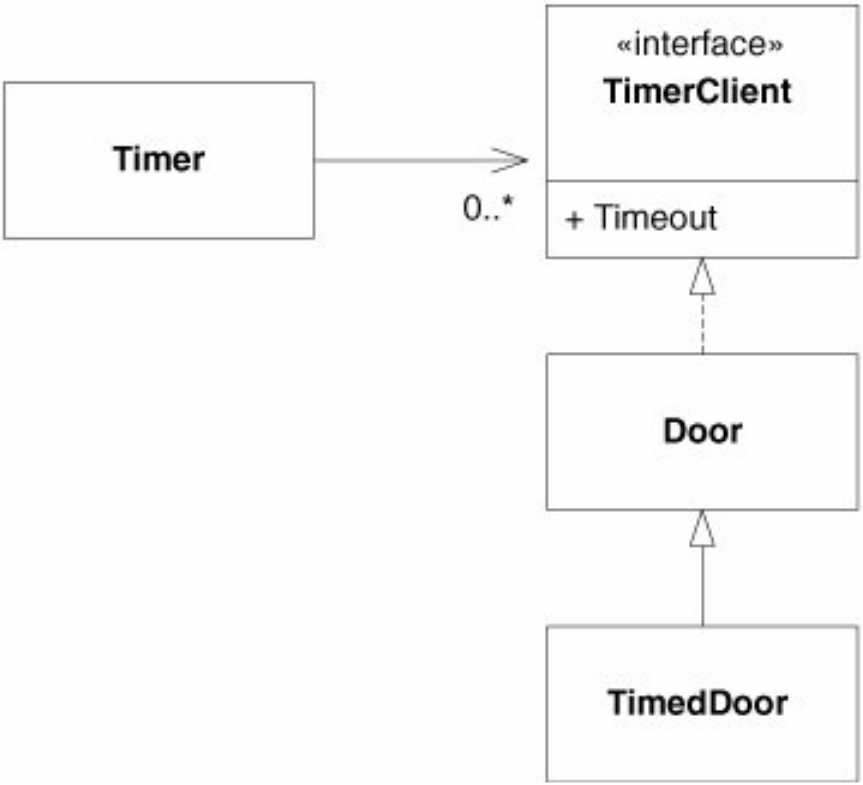
\includegraphics[scale=0.2]{ispBad}}
	\end{center}
\end{frame}

\begin{frame}[containsverbatim]
	\frametitle{Interface Pollution}
	Bad ISP implementation\\
	\begin{lstlisting}
class Timer{
    void register(int timeOut, TimerClient tc){
        ...
        Thread.sleep(timeOut);
        if(tc.isDoorOpen()){
            tc.timeOut();
        }
        ...
    }
}
	\end{lstlisting}
\end{frame}

\begin{frame}
  \frametitle{Interface Pollution}
  \begin{itemize}
	\item<+-> \textit{Door} depends on \textit{TimerClient}, its interface is polluted with timeout method of \textit{TimerClient}.. not all \textit{Door}s need this kind of coupling... 
	\item<+-> ..we could have degenerate solutions violating LSP..\\
	\item<+-> Interface is polluted with a method that does not require.. introduced to satisfy a particular need..
   \end{itemize}
\end{frame}

\section{Separate Clients Mean Separate Interfaces}
\subsection{Separate Clients Mean Separate Interfaces}
\begin{frame}
  \frametitle{Separate Clients Mean Separate Interfaces}
  \begin{itemize}
	\item<+-> \textit{Door} and \textit{TimerClient} represent interfaces that are used by completely different clients.. they should use different interfaces 
	\item<+-> Usually a change in interface implies a change in clients..
	\item<+-> But the other way around is also possible!.. a client \textbf{forces} a change in the interface..
	\item<+-> When client are forced to depend on methods don't use, are subject to changes of those methods..
	\item<+-> ..a coupling problem arise
   \end{itemize}
\end{frame}

\section{Class Interfaces versus Object Interfaces}
\subsection{Class Interfaces versus Object Interfaces}
\begin{frame}[containsverbatim]
	\frametitle{Class Interfaces versus Object Interfaces}
  \begin{itemize}
	\item<+-> \textit{TimedDoor} has two interfaces used by separate clients: \textit{Timer} and users of \textit{Door}..
	\item<+-> Those must be implemented in the same object, since implementations manipulate same data..
	\item<+-> But how to do it respecting ISP?.. How to separate interfaces when they must remain together?
	\item<+-> Answer is that client don't need to access an object through an interface; they can access it through delegation or through a base class.
   \end{itemize}
\end{frame}

\subsection{Separation Through Delegation}
\begin{frame}
  Define an object that derives from \textit{TimerClient} and delegates to \textit{TimedDoor} \\
  \frametitle{Separation Through Delegation}
  \begin{center}
	\fbox{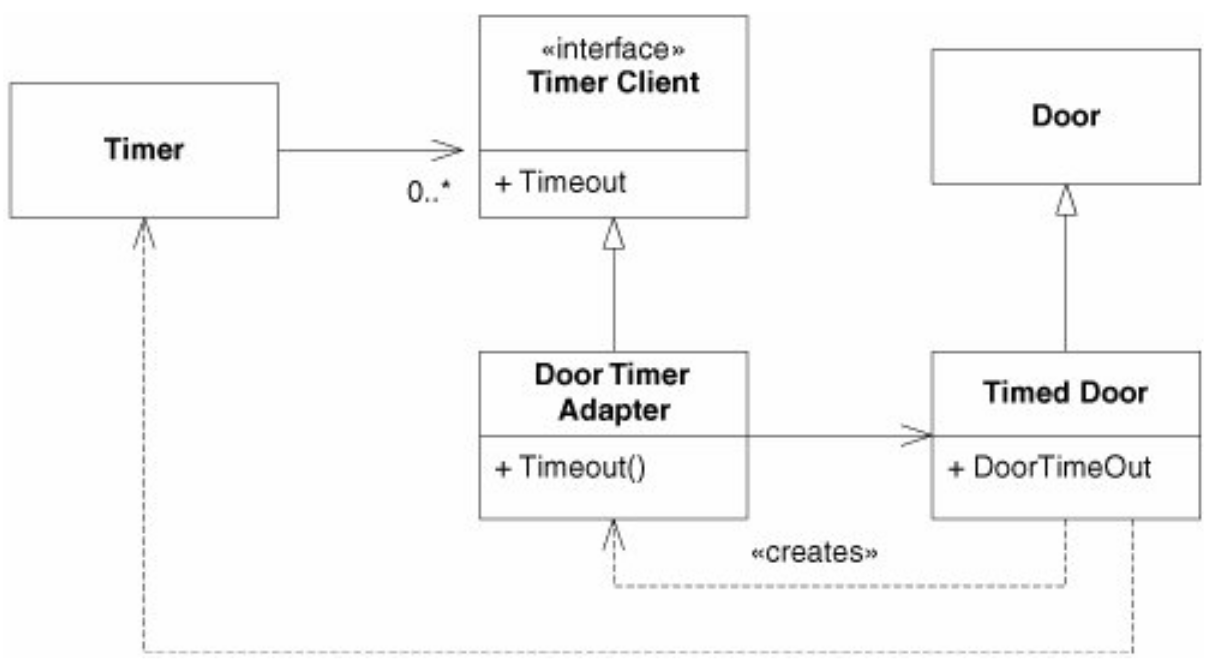
\includegraphics[scale=0.2]{doorTimeAdapter}}
	\end{center}
\end{frame}

\begin{frame}
  \frametitle{Separation Through Delegation}
  \begin{itemize}
	\item<+-> When a timer registration is needed; \textit{TimedDoor} creates a \textit{DoorTimerAdapter}
	\item<+-> When the \textit{Timer} sends the \textit{TimeOut} message to the \textit{DoorTimerAdapter} , the \textit{DoorTimerAdapter} delegates the message back to the \textit{TimedDoor}
	\item<+-> This solution is ISP compliant, prevents coupling of \textit{Door} clients to \textit{Timer}
	\item<+-> Is a general purpose solution but has a little overhead...
   \end{itemize}
\end{frame}

\subsection{Separation Through Multiple Inheritance}
\begin{frame}
  \frametitle{Separation Through Delegation}
  \textit{TimedDoor} inherits from both \textit{Door} and \textit{TimerClient} \\
  Clients use same objects through separate interfaces \\
  \begin{center}
	\fbox{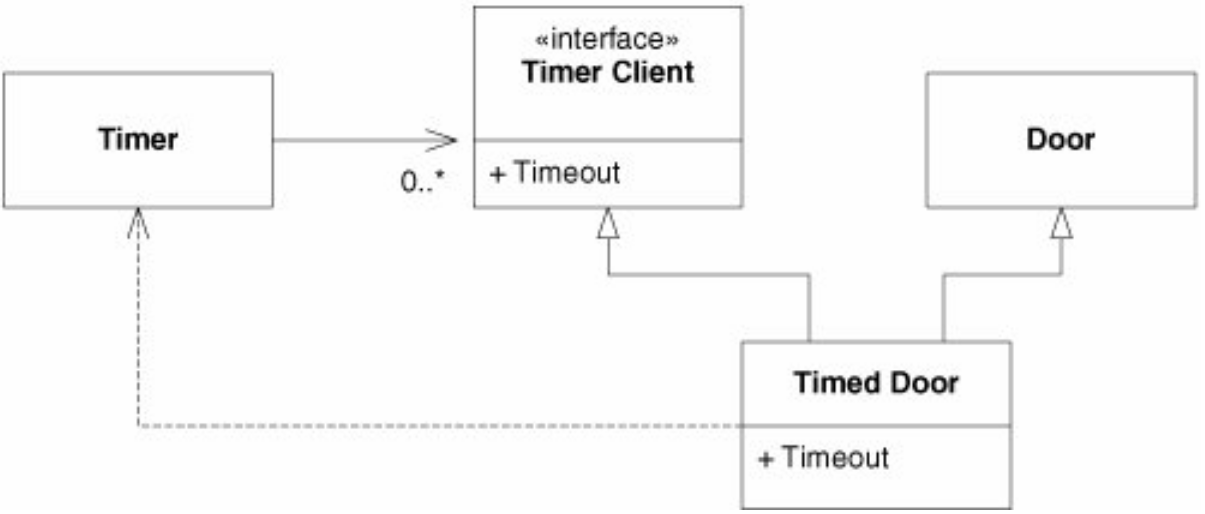
\includegraphics[scale=0.2]{multiIhn}}
  \end{center}
\end{frame}

\section{The ATM User Interface Example}
\subsection{The ATM User Interface Example}
\begin{frame}
  \frametitle{The ATM User Interface Example}
  ATM needs to be very flexible: output may be translated, showed on screen, braille or spoken.. \\
  \begin{center}
	\fbox{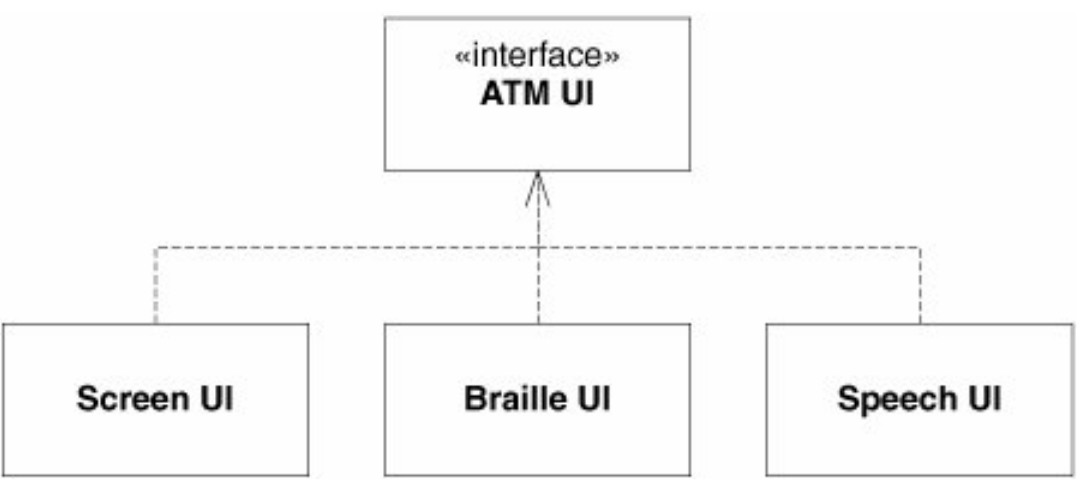
\includegraphics[scale=0.2]{atm}}
  \end{center}
\end{frame}

\begin{frame}
  \frametitle{The ATM User Interface Example}
  Moreover exist derived transaction that interact with UI.. \\
  \begin{center}
	\fbox{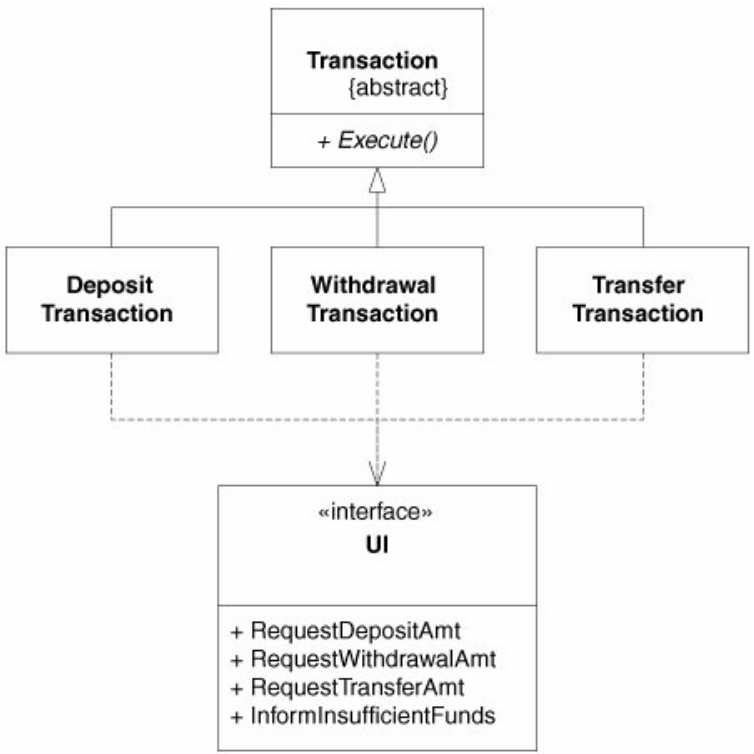
\includegraphics[scale=0.2]{transaction}}
  \end{center}
\end{frame}


\begin{frame}
  \frametitle{The ATM User Interface Example}
  \begin{itemize}
	\item<+-> Each transaction is using UI methods that no other class uses..
	\item<+-> A change occuring in a derivative can force a change in UI affecting all the other derivatives or any other UI dependent..
	\item<+-> Supposing an add of a new transaction... we need to add a method to UI also.. this implies a rebuilt of dependents of UI..
	\item<+-> Segregating UI interface into individual interfaces avoids useless coupling...
	\item<+-> ..polyadic could be better than monadic sometimes.. (?!)
   \end{itemize}
\end{frame}

\section{Conclusion}
\subsection{Conclusion}
\begin{frame}
  \frametitle{Conclusion}
  \begin{itemize}
	\item<+-> Fat classes cause bizarre and harmful couplings between their clients..
	\item<+-> A change forced by a client against a fat class, can impact against other clients of the fat class
	\item<+-> A client should depend only on methods it calls...
	\item<+-> So segregate single responsibilities in separated interfaces and merge them by inheriting if needed...
	\item<+-> In this way clients are decoupled from methods they don't invoke keeping them independent
   \end{itemize}
\end{frame}

\end{document}
